\chapter{Model Design}
\section{Introduction}
In this section, the theories and methods from Chapter 3 will be formalized into a computational model. Before doing so, the characteristics of the system under consideration will be discussed. The model will simulate the behavior of agents in a consumer-centric energy system. Section \ref{CASEnergy} will discuss whether this consumer-centric energy system is a CAS or not. Since the model is rather complex due to the large amount of agents and interactions, the explanation of the model will be done in different stages. In section \ref{Concept}, the logical process that created the final version of the model will be summarized. Since the model development happened through a few important stages, between which features got added and complexity gradually increased, an conceptual overview of these different steps will help the reader in understanding the final version of the model. In this section, the description of the model will be limited to a high-level overview of the input parameters, output parameters and agents in the environment. A more detailed description of the model will be discussed in section \ref{formalisation}. In this section, the different processes, equations and input data included in the model will be described by using the ODD protocol\footnote{The ODD protocol is a framework developed specifically for agent-based model to describe and decompose the ABM in a systematic and standardised manner}. This standard structure called the ODD protocol will be followed to make the system decomposition as straightforward and reproducible as possible.
\section{Consumer-centric energy system as a complex adaptive system?} \label{CASEnergy}
One of the main assumptions of this Thesis is that a consumer-centric energy system can be considered a complex adaptive system. This assumption can be supported by comparing the properties of a CAS with the system under consideration. First, however, the layout of the system must be presented.
\newline \newline \noindent
The system under consideration consists of a set of households and the DSO. Among the households, that are the electricity consumers, there will be two distinct groups: households that have the possibility to adopt DERs ("Replacement demand") and households that are not in the ability to adopt DERs due to logistical (i.e. households that live in apartment buildings or very remote places) or other constraints ("Residual demand"). The DSO will interact with both these groups, as can be seen in Figure \ref{Figure:split}.  
\begin{figure}[h!]
\centering
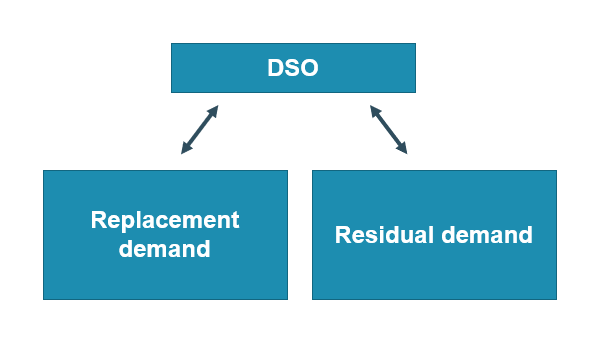
\includegraphics[width=8cm]{modelarge.PNG}
\caption{System overview}
\label{Figure:split}
\end{figure}
\noindent 
There will be multiple kinds of interactions in this system. These interactions will be both between the household with replacement demand as well as between the groups of households and the DSO. 
\newline \newline \noindent
The households with replacement demand will gradually adopt PV-battery configurations, driven by economic incentives and peer influences. The aggregate effect of all these agent-level adoptions will cause the overall DERs adoption levels to increase on a system level. This phenomenon is an form of emergent behavior, which is one of the most important characteristics of a CAS. The agents in the system will change their behavior based on changes in circumstantial factors. Households will change their attitude towards investing in DERs as the electricity price (including distribution cost), technology cost and peer influence change. The DSO will change its pricing strategy as the amount of electricity consumed will change. These changes will be an expression of adaptive characteristics on behalf of the agents. This adaptive behavior also is a cornerstone of any CAS and is very much present in the system under consideration. Since this Thesis studies the effect of different policies on the adoption of DERs and the utility death spiral, different stimuli will be introduced into the system which will influence the responses of the agents. Since these responses depend on the state a certain agent is in (wealth level, adoption characteristic, distribution tariff etc.), the responses are state-based responses. This also is an important part of a CAS.
\newline \newline \noindent
Since some of the most important characteristics of a CAS (emergence, adaption and state-based responses) will prevail in the system under consideration, it is a fair assumption to say that the energy system that the model simulates is a CAS. 
\section{Conceptual model} \label{Concept}
In this section, the model will be presented from a conceptual point of view, by gradually adding features to understand what the input-output relations of relevance are in the model. The end model of this Thesis is the result of many iterations of feature additions and intermediate evaluations, of which the final iteration will be the main point of attention in this section. A representation of this conceptual model can be found in Figure \ref{Figure:model3}.
%\begin{figure}[h!]
%\centering
%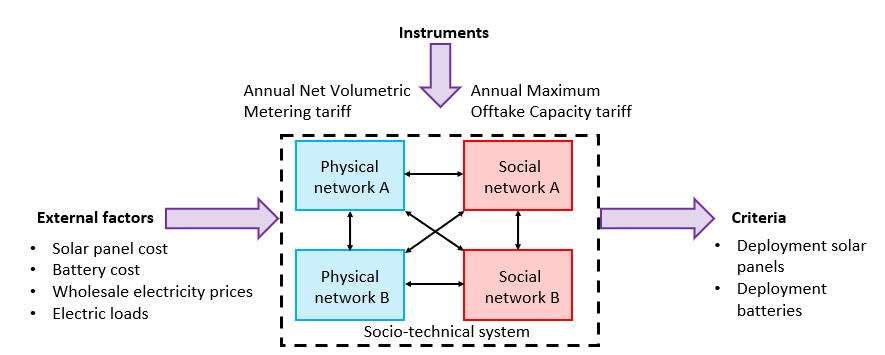
\includegraphics[width=10cm]{model1.PNG}
%\caption{Exogenous model overview}
%\label{Figure:model1}
%\end{figure}
%The independent variables are the different distribution tariffs that can be set by the grid operator. The first kind of distribution tariff is the net volumetric metering tariff. This tariff, which charges the electricity consumer a fixed distribution rate for each unit of net electricity taken from the grid, is the most common way DSOs will charge the end consumers for the usage of the distribution infrastructure. A common tariff charge is about 0.1\EUR{}/\textit{kWh}. Compared to the energy component of the overall electricity bill, this distribution cost will often be larger than the actual energy cost. 
%Another distribution tariff is the annual maximum offtake capacity tariff. For this tariff, the overall distribution cost will depend on the maximum demand on an annual basis. A common tariff charge for the capacity offtake tariff is about 9.0 \EUR{}/$kW_{peak}$. 
%\newline \newline \noindent
%Since the distribution tariffs are exogenous in this stage of the model, they remain constant throughout the simulation period. Given all these input parameters, the battery and solar PV adoption will be the output parameters. In a next stage, the interaction between the households and the DSO will be added to the model, by making the group of households interact with the DSO. A visual representation of this model can be found in Figure \ref{Figure:model2}.
%\begin{figure}[h!]
%\centering
%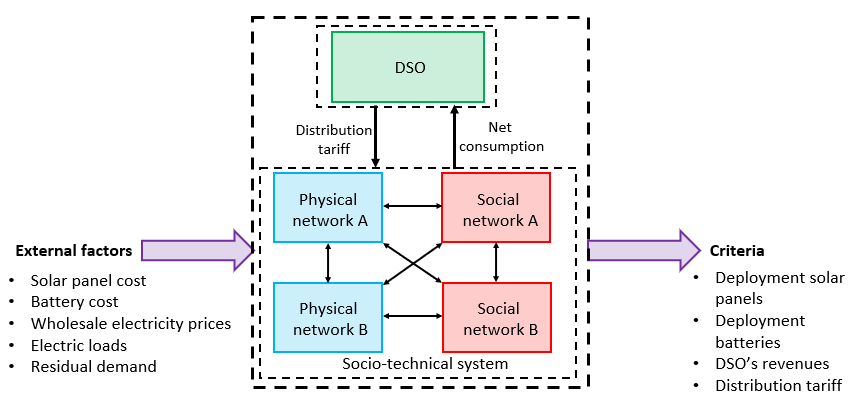
\includegraphics[width=10cm]{model2.PNG}
%\caption{Endogenous model overview}
%\label{Figure:model2}
%\end{figure}
%In addition to the aforementioned input parameters, the residual load will also have to be explicitly defined. This parameter is required to determine the extent of the utility death spiral. The distribution tariffs no longer will be constant, but their initial values will still need to be defined. As the PV and battery adoption increases and the electricity demand from the grid changes over time, the DSO will see a shift in his revenues, forcing him to adapt his pricing towards the end customers. The output parameters in this version of the model, therefore, next to the PV and battery adoption are the DSO revenues and distribution tariffs. 
%\newline \newline \noindent
%In the final version of the model, the represented model of Figure \ref{Figure:model2} is to be tested for different policies, as can be seen in Figure \ref{Figure:model3}. The policies that are to be evaluated are the feed-in tariff, net metering, net billing and battery subsidies. The data used to quantify these different adoption incentives was based on those policies being deployed in Belgium. 
\begin{figure}[h!]
\centering
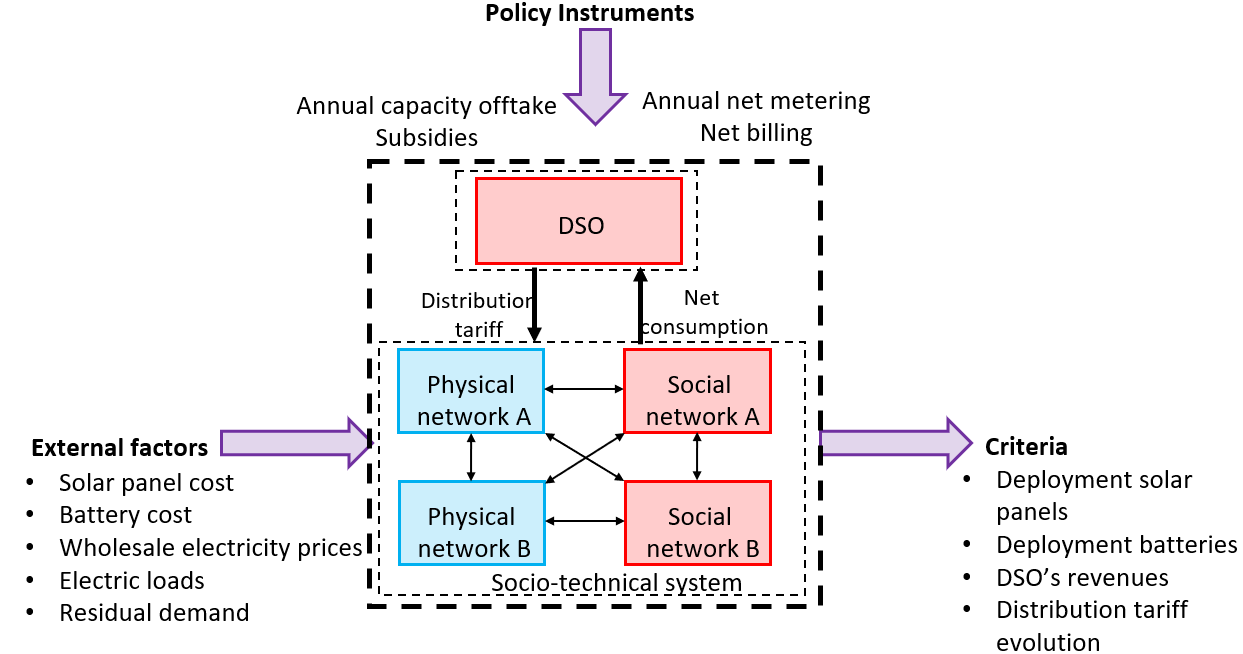
\includegraphics[width=10cm]{model3.PNG}
\caption{Policy model overview}
\label{Figure:model3}
\end{figure}
As can be seen, the exogenous input parameters to the model are the different policies considered in the Thesis: annual net metering, annual capacity offtake, net billing and battery subsidies. The external input parameters are the solar panel cost, battery cost, wholesale electricity price, electric load and residual demand of the aggregate of households. The resulting output parameters are the solar PV deployment, battery deployment and the evolution of the distribution tariff.  
\section{Model formalisation} \label{formalisation}
\subsection{Introduction}
In this section, the theories and methods that were discussed in section \ref{Prospect} and section \ref{Modeling} will be used to develop the agent-based model for simulating the DERs adoption on a household level. In doing so, a common framework for the decomposition of ABM, called the ODD framework, will be the first point of attention.
\subsection{ODD protocol}
Due to the complexity of some ABMs, a standard framework for the description of these models is a useful way to understand, decompose and reuse a model, or parts of it. The ODD protocol can serve as a structure to fulfill this task. The ODD (acronym for 'Overview', 'Design Concepts' and 'Details') is a protocol that was developed to standardize the description of agent-based and individual-based models in publications. This way, models are easier to understand and implement in later research. Within the three basic elements of the ODD protocol, there are a few sub-elements that have to be defined. Before going to the specific model development in section \ref{MODEL}, a description of the ODD protocol will be given. The sub-elements of the ODD protocol are: 
\begin{itemize}
    \item \textbf{Overview}: Purpose, entities/state variables/scales and process overview/scheduling. 
    \item \textbf{Design concepts}: Basic principles, emergence, adaptation, objectives, learning, prediction, sensing, interaction, stochasticity, collectives and observation.
    \item \textbf{Details}: Initialization, input data and submodels.
\end{itemize}
By addressing the different topics in this framework, the structure of the model under consideration can be decomposed and reported. Since the model simulates the behavior of agents in a CAS, the different characteristics discussed in section \ref{CAS} will also be a point of attention. Therefore, the different items characterizing CAS and the different parts of the ODD framework will be aligned in section \ref{development}.
\subsection{Model development} \label{MODEL} \label{development}
Concepts from CAS theory and decision making theories will now be formalized into an agent-based model. A first point of attention will be the assumptions governing the model. Subsequently, the model overview will be presented according to the items of the ODD protocol and discussing how the different characteristics of CAS theory fit into this model description. 
\subsubsection{Assumptions}
The following assumptions were made in the development of the model:
\begin{itemize} 
    \item Besides the energy and distribution component, no other parts to the electricity cost (like taxes and levies) are considered.
    \item The households will be risk seeking when facing losses and risk averse when facing gains.
    \item The households will act as prospect value-maximizing agents (subjective value optimization).            
    \item Several data sequences, like the DAM electricity prices and the load factor of the PV are exogenous. The load factor remains constant throughout the entire temporal scope of the model.
    \item The agents/households live densely enough to be able to observe what their neighbors are doing. If this was not the case, the influence of the peer effect could no longer be relied upon.
    \item The interaction between the aggregate of households and the DSO is assumed to be direct without any intermediary party like an aggregator or flexibility service provider.
    \item The nature of the household remains unchanged over time: an innovator remains an innovator throughout the entire simulation, as will laggards and all the other classes of households.
    \item The financing of the DERs is done entirely through the own means of the household. Given the very low interest rates that have been shaping the financial markets in past years, debt is virtually free and, therefore, this is a fair assumption \cite{ECB}.
     \item The households adopt on a one-off basis, meaning that no upgrades or extensions of the adopted configurations are possible.
     \item Since the focus in this Thesis is on the adoption of DERs rather than the decommissioning, the latter is not accounted for in the model.
     \item The residual load households' demand elasticity to the electricity price is assumed to be 0. This implies that for increasing network charges and electricity cost, the residential demand of these households remains the same. 
\end{itemize}
With these assumptions in mind, the model will be described using the ODD protocol, which will be done in the next section.
\subsubsection{Model Overview} \label{overview}
In this section, the ODD protocol will be used to describe the model that simulates households' DERs adoption. When discussing the different characteristics and components of the model, their relevance in the CAS framework, which was discussed in section \ref{CAS}, will also be a point OF attention.
\begin{itemize}
 %   \item \textbf{Purpose}: provide insights into how different policy instruments, like net billing, net metering, feed-in tariffs and others affect household DERs adoption and enhance the utility death spiral.
   % \item \textit{Entities}:  different agents, being the different households and the DSO
   % \item \textbf{State variables}: adoption rates of PV/Battery systems, income level and adoption type for the households. For the DSO, these state variables are the distribution tariffs and grid revenues
    %\item \textbf{Scale}: The temporal scale is 20 years (lifetime of the technology under investigation). The temporal resolution of the model is 1 year. The spatial specification are also necessary since this model will consider the peer effects of the households upon each other
   % \item \textbf{Project overview}:  describes the schedule of the different processes in the model. A high level description of the process overview can be seen in Figure \ref{fig:flow}. The underlying models that will require further discussion are the cost optimization model, the economic utility calculation, peer adoption effect (and social utility calculation) and distribution tariff variation. This part of the model discussion can be found in section \ref{submodel}. 
   % \newline 
   % \begin{figure}[h!]
        %\centering
        %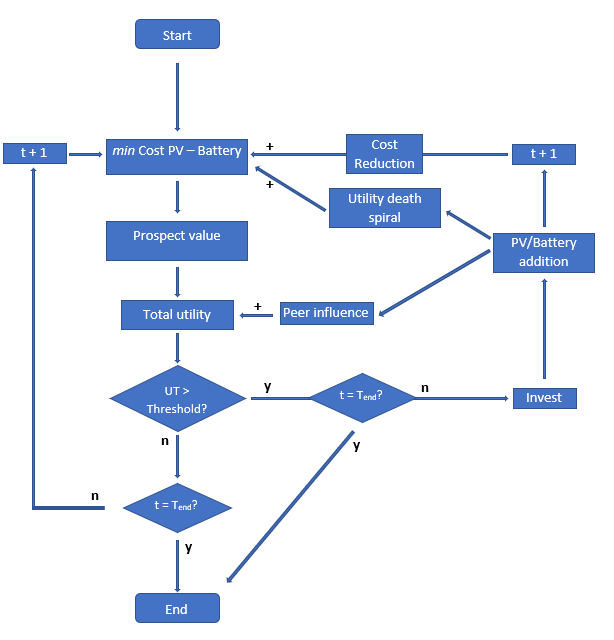
\includegraphics[width=10cm]{flowchart.PNG}
      %  \caption{Process overview of the model}
    %    \label{fig:flow}
  %  \end{figure}
    %\item \textbf{basic principles} are the implementation of cumulative prospect theory into an investment decision making model for DERs on a household level.
    %\item \textbf{emergent behavior} since the aggregate of households will gradually adopt PV-battery configurations, initially due to purely economic reasons, but gradually also due to the social utility that the peer effect will evoke.
\end{itemize}
%\newline \newline \noindent
The \textbf{purpose} of the model in this Thesis is to provide insights into how different policy instruments, like net billing, net metering and battery subsidies affect household DERs adoption and enhance the utility death spiral. In the model, the adoption of DERs, PV/battery configurations to be more specific, is simulated on a household level. The system the model considers consists of a group of several thousands of households that will interact with each other through the peer effect. Combining the social utility of this peer effect with their economic utility, households will decide whether to adopt DERs or not. The group of households will also interact with the DSO through the variation of distribution tariffs due to less electricity consumption from the grid after having adopted DERs.
\newline \newline \noindent
The \textbf{entities} of the model are the different agents, being the different households and the DSO. The \textbf{state variables} are the adoption rates of PV/Battery systems, income level and adoption type for the households. For the DSO, these state variables are the distribution tariffs and grid revenues. The \textbf{scales} of the model are both temporal and spatial. The temporal scale is 40 years (lifetime of the technology under investigation). The temporal resolution of the model is 1 year. The spatial specification are also necessary since this model will consider the peer effects of the households upon each other. The spatial scale, therefore, must be confined to an area consisting of a group of households of sufficient size to make the effects of the adoption clearly visible. This household network will be modeled using the income level distribution of the households. The \textbf{process overview} describes the schedule of the different processes in the model. A high level description of the process overview can be seen in Figure \ref{fig:flow}. The underlying models that will require further discussion are the cost optimization model, the economic utility calculation, peer adoption effect and distribution tariff variation. This part of the model discussion can be found in section \ref{submodel}. 
\newline 
\begin{figure}[h!]
    \centering
    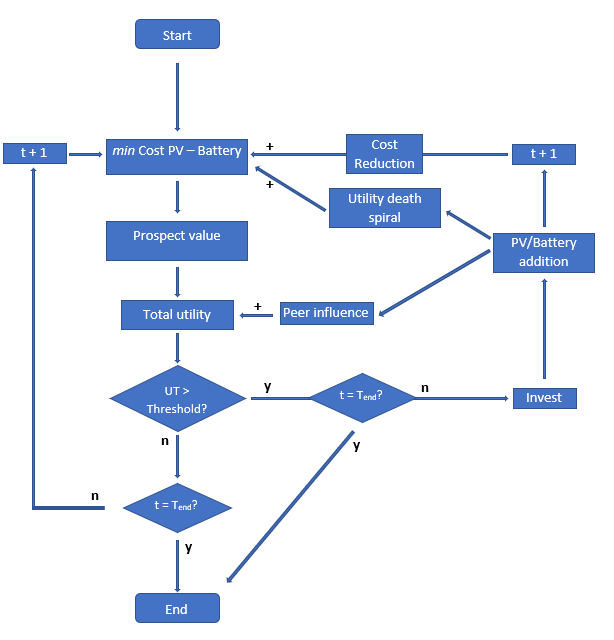
\includegraphics[width=10cm]{flowchart.PNG}
    \caption{Process overview of the model}
    \label{fig:flow}
\end{figure}
\noindent
When focusing more on the design concepts, the \textbf{basic principles} are the implementation of cumulative prospect theory into an investment decision making model for DERs on a household level. In doing so, the assumption is that individuals or households will not make decisions on a rational basis, but will incorporate risk aversion factors in their decision making. This model will incorporated into an agent-based model to describe the investment decision making in electricity generation assets. Prospect theory is used to capture non-rational behavior of households/individuals. In addition, social utility is also added in the utility calculation to account for non-economic decision variables. 
\newline \newline \noindent
Each agent will adapt his behavior to the situation at hand. Two parameters will cause the households to adapt their behavior: the economics of the technology and the peer effect. If the technology, be that PV or batteries, becomes cheaper because of further scaling or innovation, the utility of a certain configuration will increase, thereby causing the household to change its views on the technology, making its behavior change. If, on the other hand, many neighbors of a certain household adopt PV/battery installations, the peer effect will cause the social utility to increase, making the non-adopting households change their views on the adoption of the DERs, thereby making them adapt their behavior. The DSO will gradually adapt his behavior (by adapting the distribution tariffs) as the adoption of DERs increases and the utility death spiral starts manifesting itself. Note that this adaptation is very important in the overall ODD protocol, since it is one of the core characteristics of a CAS (see section \ref{CAS}). 
\newline \newline \noindent
Another  important characteristics of the CAS, emergent responses, will be present in the model. The model will show \textbf{emergent behavior} since the aggregate of households will gradually adopt PV-battery configurations, initially due to purely economic reasons, but gradually also due to the social utility that the peer effect will evoke. However, since the amount of households and installable capacity is limited, this emergent behavior in the model will saturate to a certain point, which will be a point of widescale PV adoption when sudden emergence of PV adoption no longer is possible. The agents in the system will show a different behavior towards their adoption patterns. Whereas the adoption will at first purely be motivated by economic utility, this will gradually become motivated by both economic and social utility.
\newline \newline \noindent
The \textbf{objectives} of the agents in the model will depend on what kind of agent is being considered. The objectives of the households are to minimize the costs (or under behavioral finance, the 'perceived cost') of  electricity consumption. For the DSO, the objective is to recover the costs it had to incur to construct and maintain his infrastructure. Although the agents in the model will show an adaptive behavior, there will be no additional \textbf{learning} features exhibited by the households other than the adaptations to the situation as it presents itself at any given moment in time. 
\newline \newline \noindent 
Another important property of a CAS (see section \ref{CAS}) is prediction. The \textbf{predictive} capacities of the households will also be limited, since all they do is predict what the NPV and payback period is of the PV/battery configuration. The different agents in the system will \textbf{sense} different parameters. The behavior of the agents will be influenced by the electricity prices (including the distribution costs), the load factor of the PV and the adoption of PV by the neighbors of the agent. The DSO will adapts his behavior according to the net amount of electricity that will be drawn from the grid and the residual demand (i.e. demand that cannot be substituted by PV or another DERs). 
\newline \newline \noindent
Agents will \textbf{interact} with each other. If more agents decide to adopt PV, thereby reducing the net demand for electricity, the DSO will react by increasing the distribution tariff on the electricity sold. In this process, the different agents are interacting with each other (i.e. they will adapt their behavior as a reaction to what other agents do). The households, however, will also interact with each other. Due to the peer effect, the adoption by other households becomes more likely if a neighboring households installs a PV-battery system. 
\newline \newline \noindent
Since there is a level of uncertainty created in some variable, like the price of electricity, load factor, or price of the technology, this model does integrate some \textbf{stochastic} processes. This uncertainty is incorporated through the projection of various random scenarios of different parameters. Therefore, the discussion of model simulation results will not be done using those of a single simulation. Rather, a Monte Carlo approach will be done to systematically analyze the results of a large batch of results, to get as complete a picture as possible of the internal mechanics of the model. This will require some computation time, but will give a more adequate representation of the model results. As mentioned earlier, there are several agent interactions in the system (i.e. household-household and household-DSO). Note how this visualisation aspect aligns with the computer simulation characteristics of the CAS (see section \ref{CAS})
\newline \newline \noindent
In the interaction between the group of households and the DSO in the utility death spiral, the households form an aggregation of agents that will collectively affect the state and behavior of the system, since the distribution tariff will be adapted through this \textbf{collective} behavior. To evaluate the model, the \textbf{observation} parameters will depend on the agent in the system. When looking at the households, the important parameters are the PV and battery adoption, social and total utility and the payback period of the technology, as well as the evolution of the NPV. On a system level, the PV and battery adoption levels are also an important observation parameter. For the DSO, the relevant parameters are the distribution tariff and the change in its revenue stream. 
\newline \newline \noindent
The model was \textbf{initialized} as follows: no households with any DERs, all electricity consumption from the grid and a volumetric or capacity distribution tariff. These initial conditions could also be changed to a partial adoption initial condition (for instance  30\% adoption of solar PV in a neighborhood), but since the focus in this Thesis is on the adoption process of the DERs, it is more interesting to simulate the entire adoption from scratch. The primary \textbf{input data} of the model should be the electricity price of the Day-ahead market (DAM) (Figure \ref{fig:price}) and the residential demand (Figure \ref{fig:demand}). 
%\begin{figure}[h!]
%\centering
%\begin{subfigure}{\textwidth}
%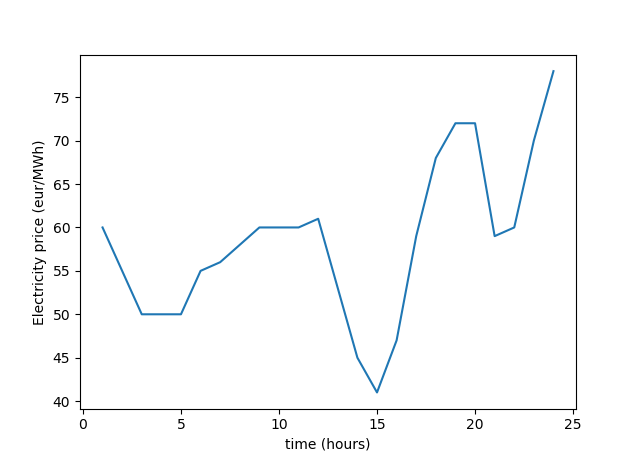
\includegraphics[width=7cm]{price.png}
%    \caption{DAM electricity price (\EUR{}/MWh)}
%    \label{fig:price}
%    \end{subfigure}
%\begin{subfigure}{\textwidth}
%    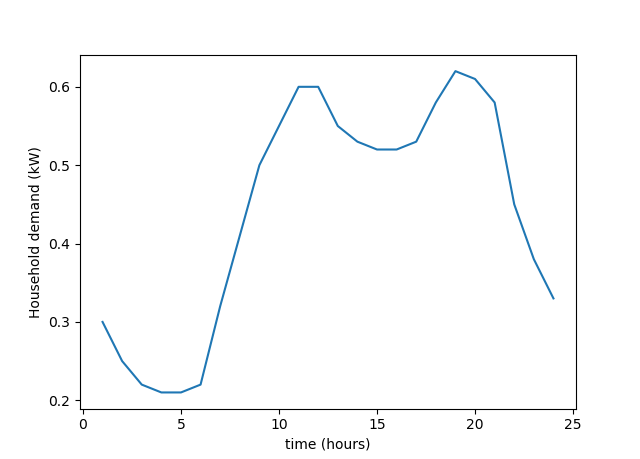
\includegraphics[width=7cm]{Demand.png}
%    \caption{Residential load profile (kW)}
%    \label{fig:demand}
%\end{subfigure}
%\label{fig:fig}
%\end{figure}
%\noindent
So far though, households are not charged hourly electricity prices. Usually, households are charged two tariffs: a night and day one. In all these cases, though, it is important to stress that varying price profiles could make the results of this model deviate from their intended purpose. The main focus of this Thesis is to determine how PV adoption and the utility death spiral occur as a result of economic and social incentives. By introducing sources of noise into the model, which can come in the form of varying electricity prices, varying PV prices or any other, therefore, it becomes increasingly difficult to observe the input-output relations of the model. Hourly electricity prices on a residential level could incentivize the households to adopt PV-batteries with the sole purpose of doing energy arbitrage between peak and low demand hours, rather than the economic and social incentives that are considered in this model. To avoid this hidden adoption incentive, electricity prices will assumed to be constant throughout an entire year. The price can still change in between years. If in the future hourly electricity prices are to be charged to households, this additional phenomenon will have to be accounted for in future work. 
\newline \newline \noindent
Since this model also concerns a PV system, the load factor also is an important set of input data. A representation of the load factor data that is to be used in this model can be found in Figure \ref{fig:LF}:
%\begin{figure}[h!]
%    \centering
%    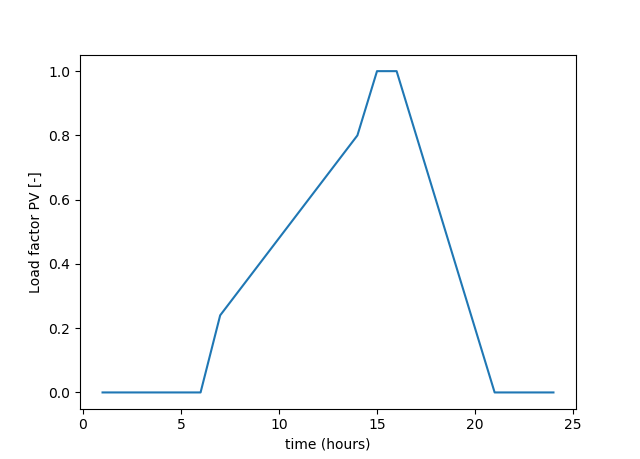
\includegraphics[width=7cm]{LF.png}
%    \caption{Load factor of the PV [-]}
%    \label{fig:LF}
%\end{figure}
%\noindent
The data shown in Figures \ref{fig:price},  \ref{fig:demand} and \ref{fig:LF} is a weighted average of a set of representative days to account for the annual profile of the residential demand, DAM electricity price and load factor. Using twelve standard profiles that jointly represent the most important characteristics of an annual electricity price, residential demand and PV load factor profile. Each of these days will have a representative weight to account for the annual profile. When performing calculations with this data, the amount of computations will remain limited, since the results of the calculations using representative days data can be multiplied with the associated weight, rather than performing the calculations with the entire annual data. An important side note to the data in Figure \ref{fig:demand} is that this data will vary as a function of the income/wealth of the household, which will be discussed in a subsequent paragraph.
\newline \newline \noindent
In addition to the exogenous data strings represented in Figures  \ref{fig:price}, \ref{fig:demand} and \ref{fig:LF}, some additional data will be required. The first important set of data is related to the technology cost. Since these technologies are also emerging technologies that are undergoing decreases in capital cost (see section \ref{Trends}), the assumed annual price decrease also is an important factor that should be included. This data can be found in table \ref{tab:PVbat}. The solar panel data on capital and operational costs can be found from the IEA data in Table \ref{table:1}. The value for the EU will be selected for the solar PV data: $\$1,300$ per $kW$.  The complementary maintenance cost will be included ($\$20$ per \textit{kW}). The battery data comes from the cost estimaetes by the NREL \cite{batdata}. On average, the cost of the battery is 500 $\frac{\$}{kWh}$.
\begin{table}[h!]
    \centering
    \begin{tabular}{||c|c|c|c||}
    \hline 
          \textit{\textbf{Technology}} & \textit{Capex} ($\frac{\$}{kW(h)}$) & \textit{Opex} ($\frac{\$}{kW(h)-year}$) & \textit{Capex decrease} (\%)\\
         \hline 
         \hline
          \textbf{\textbf{PV}} & 1,300 & 10 & 3\\
          \textbf{\textbf{Battery}} & 500 & 9 & 5\\
          \hline 
    \end{tabular}
    \caption{Cost overview of PV \& battery}
    \label{tab:PVbat}
\end{table}
The capital costs of the PV are assumed to decrease by 3\%,. This value is the result of an estimation based on the capital cost decrease projection of the PV in Table \ref{table:1}: the capital cost is expected to decrease by 41\% by 2040, which results in an annual cost decrease of 2.5 - 3\%. Cost decreases for residential storage facilities are more challenging to obtain, but since this technology will still undergo a substantial expansion, the annual cost decrease is going to be higher. In this Thesis, a cost decrease of 5\% is assumed. This may appear to be a high value, but when comparing this to the annual cost decrease for the lithium-ion technology in recent years (see Figure \ref{Figure:bloom}), this cost decrease seems reasonable. One point of attention that must be met here, however, is that this cost decrease of PV and battery technology hinges on the ability of the DER manufacturers to keep up with this demand. The overall demand for PV is expected to steadily increase the cumulative PV capacity (see Figure \ref{Figure:PVfut}), but if this demand systematically exhaust the limited supply, the cost of PV and other DER will no longer decrease as projected. Depending on the evolution of the PV manufacturers, this assumption will have to be adjusted in the future. 
\newline \newline \noindent
The additional costs the households will have to incur for the installation of the PV-battery system include the cost of the converter, cables, protective equipment and installation labour cost. For each configuration, this cost is assumed to be fixed (\EUR{}1200\footnote{Based on the recent installation of PV panels at the authors' home}). With all the different cost components known, there will be a set of available configurations. In reality, there are many possible configurations for households to adopt. Selecting a PV-battery configuration, nonetheless, is always a discrete process, since both PV panels and batteries come in modules of some minimal capacity. The possible configuration can, therefore, be approximated by a limited set of options, as can be seen in table \ref{tab:config}.
\begin{table}[h!]
    \centering
    \begin{tabular}{||c|c|c||}
    \hline 
          \textbf{\textit{Option}} & \textit{PV capacity} $(kW_p)$ & \textit{Battery capacity} $(kWh)$\\
         \hline 
         \hline
          1 & 1.5 & 0.0\\
          2 & 1.5 & 2.0\\
          3 & 2.5 & 0.0\\
          4 & 2.5 & 2.0\\
          5 & 4.0 & 0.0\\
          6 & 4.0 & 2.0\\
          7 & 4.0 & 5.0\\
          \hline
    \end{tabular}
    \caption{Overview of PV-battery configurations}
    \label{tab:config}
\end{table}
Note how for each of the PV sizes, there will be the possibility of adopting both a PV with or without battery (of \textit{2.0 kWh}). For the largest PV system, there will also be the possibility to adopt a larger battery of \textit{5.0 kWh}. Each household will have to choose from one of these configurations when it wants to invest. This set of options is, of course, very limited. In reality, the number of possible configurations will be larger, but not extremely large, since the decision process in PV-battery systems will always be a bit of a discrete process. 
\newline \newline \noindent
The maximal charging/discharging power of the batteries can be determined by looking at different options available. By examining the different options laid out by Clean Energy Reviews, the maximal power output of residential batteries is roughly equal to $0.5*E_{BAT}$ \cite{batpower}. The charging power will, therefore, be $1.0kW$ for the $2.0 kWh$ battery and $2.5 kW$ for the $5.0 kWh$ battery. As a final note, no self-leakage and discharge losses are assumed. 	
\newline \newline \noindent
As was discussed earlier, the demand of the households will depend on the levels of wealth of the household. In Figure \ref{fig:wealth} the estimated financial wealth distribution of all households in Belgium can be seen. This data was estimated by combining the financial wealth of the individuals in Belgium and the distribution between different population classes \cite{wealthdata,wealthdata2}. According to this distribution, the demand will deviate from the data presented in Figure \ref{fig:demand}.
\begin{figure}[h!]
    \centering
    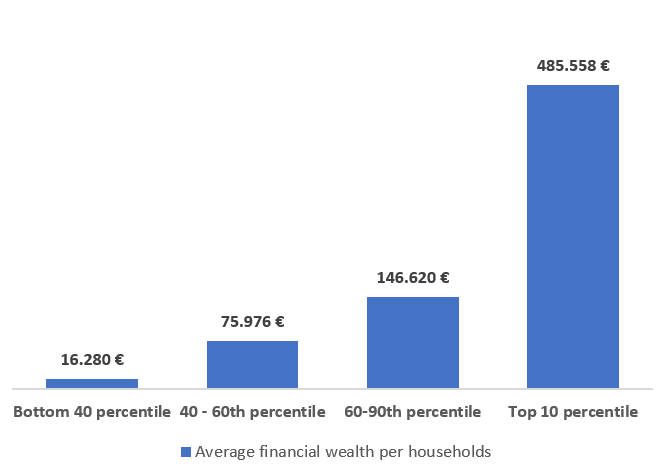
\includegraphics[width=8cm]{incomedist.PNG}
    \caption[Distribution of financial wealth]{Distribution of financial wealth \cite{wealthdata,wealthdata2}}
    \label{fig:wealth}
\end{figure}
\newline
The lowest wealth class, which accounts for 40\% of the overall population, is assumed to have a demand profile like Figure \ref{fig:demand}, only at a 20\% lower average. The subsequent wealth class, accounting for a fifth of the overall population (40-60\%), is assumed to have a demand profile that corresponds exactly to the one in Figure \ref{fig:demand}. The second to last income class, accounting for the 60th to 90th percentile of the wealth distribution, will have a demand profile that is on average 20\% higher than the standard one. The final wealth class, being the final 10\% of all the households, will have a demand profile 50\% higher than the average profile. Besides a distribution according to income, the households will also be classified according to their willingness to innovate, which will be discussed in Section \ref{submodel}. Note that this assumption is only valid if the household size is uniform (i.e., each households has the same number of members). In reality, however, poorer households tend to have more members, causing their aggregate electricity demand to be larger. This level of granularity in the household data, however, is beyond the scope of this Thesis.  
\newline \newline \noindent
As mentioned before, there are several \textbf{submodels} that are to be used in this model. These submodels include the optimization model to minimize the costs of the PV-battery configuration, the implementation of cumulative prospect theory to determine the economic utility, the peer effect to determine the social utility, the Monte Carlo simulation to capture uncertainty and the interaction between the net demand and distribution tariff for the DSO. These different submodels will be elaborated upon in section \ref{submodel}.  
\subsection{Submodels} \label{submodel}
In this subsection, there will be an overview of the submodels incorporated into the agent-based model. These submodels are the cost minimization of the PV/battery system, distribution cost evolution, economic utility, social utility implementation, uncertainty in the model and overall utility computation.
\subsubsection{Cost minimization}
This submodel, which is the first one encountered in the process schematic, will serve as a way to determine the minimal cost of the operation of PV-battery configurations. Since the optimal cost depends on the policy under consideration, the different optimization problems will be discussed.
\newline \newline \noindent
For the \textbf{annual net metering} case, the objective function is:
\begin{equation}
    min\{\sum_{t=1}^{8760} \lambda_{DAM}[t]*d[t] + dist_{net}*q_{net}\}
\end{equation}
With 
\begin{equation} \label{qnet}
    q_{net} = max\{\sum_{t} q[t] , 0 \}
\end{equation}
\noindent   
And $dist_{net}$ the net volumetric distribution tariff. For the \textbf{annual capacity offtake} case, the objective function is:
\begin{equation}
    min{{\sum_{t=1}^{8760} \lambda_{DAM}[t]*d[t]}} + dist_{cap}*q_{cap}
\end{equation}
With 
\begin{equation}
    q_{cap} = max\{ \forall t, [q[t],0]\}
\end{equation}
And $dist_{cap}$ the annual capacity offtake tariff. For the \textbf{net billing} case, the objective function is equal to:
\begin{equation} \label{voleq}
        min\{\sum_{t=1}^{8760} \lambda_{DAM}[t]*i[t] + \alpha_{DAM}[t]*e[t]  + dist_{var}*q_{net}\}
\end{equation}
With $\alpha_{DAM}[t]$ the injection tariff for the prosumer,  $i[t]$ the imported electricity (i.e. the offtake) and $e[t]$ the exported electricity (i.e. injection). As was reported by de Villena et al., the grid injection in the net billing case is not constrained \cite{Regulation}. Note that these injections and offtake can be calculated as:
\begin{equation} \label{rvw1}
	i[t] = q[t]*y_1[t]
\end{equation}
And
\begin{equation} \label{rvw2}
	e[t] = (-q[t])*y_2[t]
\end{equation}
Note that in the case of the net billing, a mixed-integer approach will be required, with $y_1[t]$ and $y_2[t]$ the binary decision variables:
\begin{equation} \label{rvw3}
	y_1[t] + y_2[t] = 1
\end{equation}
With
\begin{equation} \label{rvw4}
\{y_1[t], y_2[t]\} \: \epsilon \: \{0,1\}
\end{equation}
%This optimization is performed using the input data for electricity prices (constant value for 0.06\EUR{}/\textit{kWh}), residential demand (Figure \ref{fig:demand}) and load factor for the PV (Figure \ref{fig:LF}). The optimization problem will be a minimization problem with the electricity cost as objective function. The objective function, which is the cost function for electricity taken off the grid, consists of two components: an energy component and a distribution/transportation component. Depending on the network charge (volumetric or capacity-based) or policy (net metering, net billing and battery subsidies), there will be a difference in the optimization problem. The first kind of network charge is the so-called net volumetric distribution tariff $dist_{net}$, since the DSO will charge the consumer a fixed rate per \textit{kWh} of electricity taken from the grid. A common rate for this tariff is between 0.1 \EUR{}/\textit{kWh} and 0.2 \EUR{}/\textit{kWh}. If this network charge is applied, the distribution cost for a households on an annual basis will be:
%\begin{equation} \label{distnet}
%    distcost_{annual} =  dist_{net} * q_{net}
%\end{equation}
%With 
%\begin{equation} \label{qnet}
%    q_{net} = max\{\sum_{t} q[t] , 0 \}
%\end{equation}
%\noindent   
%The other distribution tariff design is the capacity distribution tariff. This tariff is to be based on the maximum power capacity that a consumer draws from the grid on an annual basis. This tariff, therefore, can be determined using the maximal load:
%\begin{equation}
    %q_{cap} = max\{ \forall t, [q[t],0]\}
%\end{equation}
%Given a certain fixed distribution tariff for this capacity offtake, the distribution cost will be given by:
%\begin{equation} \label{qcap}
%    distcost_{annual} = dist_{cap}*q_{cap}
%\end{equation}
%These two distribution tariffs will are to be implemented into the overall electricity cost. As mentioned earlier, there are two (major) components to the electricity bill: an energy component and distribution component. The energy component can be calculated as:
%\begin{equation}
%    {{\sum_{t=1}^{8760} \lambda_{DAM}[t]* d[t]}}
%\end{equation}
%For the net metering case, with $\lambda_{DAM}[t]$ the hourly electricity price on the DAM and $d[t]$ the power demand of a household without any DERs. For the net billing case, the energy component becomes
%\begin{equation} \label{voleq}
%      \sum_{t=1}^{8760} \lambda_{DAM}[t]*i[t] + \alpha_{DAM}[t]*e[t]
%\end{equation}
%With $\alpha_{DAM}[t]$ the injection tariff for the prosumer,  $i[t]$ the imported electricity (i.e. the offtake) and $e[t]$ the exported electricity (i.e. injection). With all the components of the electricity cost known, the objective function for the different policies can be formulated. These policies are the annual net metering, annual capacity offtake, net billing and battery subsidies. 
%\newline \newline \noindent
%The overall cost function for the \textbf{annual net metering} case is: 
%\begin{equation}
%    min\{\sum_{t=1}^{8760} \lambda_{DAM}[t]*d[t] + dist_{net}*q_{net}\}
%\end{equation}
%Where the following constraints must taken into account:
%\begin{equation}
%    q_{net} \geq \sum_t d[t]
%\end{equation}
%\begin{equation}
%    q_{net} \geq 0
%\end{equation}
%For the \textbf{annual capacity offtake} case, the cost equation becomes:
%\begin{equation}
%    min{{\sum_{t=1}^{8760} \lambda_{DAM}[t]*d[t]}} + dist_{cap}*q_{cap}
%\end{equation}
%Where the following constraints must be taken into account:
%\begin{equation}
%        \forall t: q_{cap} \geq d[t]
%\end{equation}
%\begin{equation}
%    q_{cap} \geq 0
%\end{equation}
%These cost functions are valid until the start of the model simulation, since we assume that no DERs adoption will occur until the model simulation commences. In the cost function, the economic effects of the PV-battery configuration must be accounted for. Since the PV can both provide residential power and charge the batteries for later consumption, the overall power taken from the grid will be lower. Preferably, this power is drawn from the grid when electricity prices are low and the household is self-sufficient when the electricity prices are high. To formalize this cost minimization, the objective function for the problem must be slightly adapted. For the \textbf{annual net metering case}, this objective function for the cost is:
%\begin{equation}
 %       min\{\sum_{t=1}^{8760} \lambda_{DAM}[t]*q[t] + dist_{net}*q_{net} \}
%\end{equation}
%\singlespacing \noindent
%With $q[t]$ the net power demand of the household. This net power demand is the amount of power that will be drawn from the grid on an hourly basis if a PV-battery configuration is installed. As was reported by de Villena et al., if the export exceeds the import, the excess will not be compensated \cite{Regulation}. In this Thesis, this applies to the distribution component but not to the energy component of the objective function. Note that if the interaction between the households and DSO (and the subsequent utility death spiral) is taken into account, the objective function will change to:
%\begin{equation} \label{voleq}
%        min\{\sum_{t=1}^{8760} \lambda_{DAM}[t]*q[t] + dist_{net,var}*q_{net} \}
%\end{equation}
%In this structure, the endogenous distribution tariff will change on an annual basis due to the change in net grid offtake, thereby %enhancing the utility death spiral. For the capacity tariff mechanism, the objective function will become:
%\begin{equation} \label{capeq}
%    min\{\sum_{t=1}^{8760} \lambda_{DAM}[t]*q[t] + dist_{cap,var}*q_{cap}\}
%\end{equation}
%\noindent
%In the case of \textbf{net billing}, the prosumer will be charged differently for the electricity he consumes from the grid and the %electricity he will inject into the grid. This will change the objective function to:
%\begin{equation} \label{voleq}
%        min\{\sum_{t=1}^{8760} \lambda_{DAM}[t]*i[t] + \alpha_{DAM}[t]*e[t]  + dist_{var}*q_{net}\}
%\end{equation}
%With $\alpha_{DAM}[t]$ the injection tariff for the prosumer,  $i[t]$ the imported electricity (i.e. the offtake) and $e[t]$ the exported electricity (i.e. injection). As was reported by de Villena et al., the grid injection in the net billing case is not constrained \cite{Regulation}. Note that these injections and offtake can be calculated as:
%\begin{equation} \label{rvw1}
%	i[t] = q[t]*y_1[t]
%\end{equation}
%And
%\begin{equation} \label{rvw2}
	%e[t] = (-q[t])*y_2[t]
%\end{equation}
%Note that in the case of the net billing, a mixed-integer approach will be required, with $y_1[t]$ and $y_2[t]$ the binary decision variables:
%\begin{equation} \label{rvw3}
%	y_1[t] + y_2[t] = 1
%\end{equation}
%With
%\begin{equation} \label{rvw4}
%\{y_1[t], y_2[t]\} \: \epsilon \: \{0,1\}
%\end{equation}
%With regards to the offtake and injection tariff, it is important that the injection tariff remains smaller than the the offtake tariff, added the constraint:
%\begin{equation} \label{rvw5}%
%	\lambda_{DAM}[t] > \alpha_{DAM}[t]
%\end{equation}
%\noindent
The modeling approach for the net billing policy, therefore, is a mixed-integer one. This choice of modeling was made based on the available software packages as well as ease of implementation purposes. For the \textit{battery subsidies} policy, the objective function needs no adjustments, since this policy will reduce the capital cost of the batteries, which does not fall under the objective function. Since the battery subsidies are independent of the network charge or energy remuneration, they could be combined with any of the aforementioned policies. Since the most common policy at the time this Thesis still was the annual net metering, the battery subsidies will be based on this policy. The relevant equation for the cost calculation for the battery subsidies is, therefore, Equation \ref{voleq}.
\newline \newline \noindent
With the objective functionSZ defined, some boundaries to the possible solutions must be defined. There will be several constraints limiting the potential solutions to the problem. First and foremost, the energy balance in the household must be maintained, as is defined in Equation \ref{1}. The net demand $q[t]$ is equal to the inflexible demand of the household $d[t]$ minus the solar panel electricity production $pv[t]$ and the discharge of the battery $dch[t]$ (since these can substitute electricity consumption of from the grid), plus the battery charge $ch[t]$ (since electricity is required to charge the battery). Secondly, the energy balance in the battery must be respected at all times, as is defined in Equation \ref{2}. For any period of time, the energy level in a battery must be equal to the energy level of the previous period, combined with the charging and discharging that happens over the course of the period. Note that the charging and discharging efficiencies $\eta_{ch}$ and $\eta_{dch}$ must be taken into account in this energy balance. Since this equation must be valid over the entire 24 hours of the day, the energy level in the first period of then day is the result of the charging and discharging between the last period of the previous day and the first period of the the following day, which is defined by Equation \ref{20}. Equations \ref{3} and \ref{4} constrain the operation of the PV panel. Since the production of the solar panel is limited by the amount of solar irradiation, which varies throughout the day, the load factor (LF) of the solar panel will also vary throughout the day, thereby dictating the PV production (Equation \ref{3}). Since the maximal production of the solar panel occurs at $LF = 1$, or $pv[t] = PV_{Max}$, the production of the PV panel is limited to this level, as Equation \ref{4} shows. The charging and discharging of the batteries is limited to a certain power level since the battery capacity would otherwise deteriorate too quickly. Equations \ref{5} and \ref{6} show how both these power flows are limited, taking into account the charging and discharging efficiencies. Besides the power flow to and from the batteries, the energy levels in the batteries must also be limited. Since a battery will rarely be charged to its full capacity and will not be depleted to an empty state, there will a maximal en minimal energy level imposed on the operation of the battery. This is represented in Equations \ref{7} and \ref{8}. As a final set of constraints, the PV production, battery charging and battery discharging remain positive, which is represented in Equations \ref{9}, \ref{10} and \ref{11}. The overview of the constraints will, therefore, be:
\begin{equation} \label{1}
    q[t] = d[t] - pv[t] + ch[t] - dch[t]    
\end{equation}
\begin{equation} \label{2}
    t = 1:23: \;\;\; e_{BAT}[t+1] = e_{BAT}[t] + ch[t]*\eta_{ch} - dch[t]*\frac{1}{\eta_{dch}}
\end{equation}
\begin{equation} \label{20}
    t = 24: \;\;\;\;\;\;\;\;\;\;\;\;\; e_{BAT}[1] = e_{BAT}[t] + ch[t]*\eta_{ch} - dch[t]*\frac{1}{\eta_{dch}}
\end{equation}
\begin{equation} \label{3}
    pv[t] = LF_{PV}[t]*PV_{Max}
\end{equation}
\begin{equation} \label{4}
    pv[t] \leq PV_{Max}
\end{equation}
\begin{equation} \label{5}
    ch[t]*\eta_{ch} \leq P_{Max}^{ch}
\end{equation}
\begin{equation} \label{6}
    dch[t]*\frac{1}{\eta_{dch}} \leq P_{Max}^{dch}
\end{equation}
\begin{equation} \label{7}
    e_{BAT}[t] \leq E_{Max}^{BAT}
\end{equation}
\begin{equation} \label{8}
    e_{BAT}[t] \geq E_{Min}^{BAT}
\end{equation}
\begin{equation} \label{9}
    pv[t] \geq 0
\end{equation}
\begin{equation} \label{10}
    ch[t] \geq 0
\end{equation}
\begin{equation} \label{11}
    dch[t] \geq 0
\end{equation}
These constraints must all be taken into account in the optimization problem. Note that for the net billing policy, an additional constraint must be accounted for:
\begin{equation} \label{rvw5}
	\lambda_{DAM}[t] > \alpha_{DAM}[t]
\end{equation}
Within the feasible region created by these constraints, an optimal value for $q[t]$, and therefore also the annual savings, can be found.
\subsubsection{Distribution cost evolution}
The DSO will adapt its pricing for the end customer to recover the costs incurred to maintain the grid. Given a certain revenue $R$:
\begin{equation}
    R = dist_{var,t}*Vol_t
\end{equation}
With $dist_{var,t}$ the variable distribution tariff charged to the customers at a certain point in time and $Vol_t$ the volume of electricity sold on the grid at the same time, the DSO will not allow this revenue to decrease since he needs to recover his costs. The revenue, therefore, must at least remain constant. It is important to mention, however, that the electricity sold $Vol_t$ consists of two parts: a portion that can be substituted by DERs (adoption load $Vol_{ad,t}$, which will vary as a function of DERs adoption and time) and a portion that cannot be substituted by DERs (residual load $Vol_{res}$, which is assumed to remain constant). The revenue will therefore become equal to:
\begin{equation}
    R = dist_{var,t}*(Vol_{ad,t} + Vol_{res})
\end{equation}
Since the revenue and residual load are assumed to remain constant and the adoption load is the only variable in this equation, the distribution tariff in subsequent periods is equal to:
\begin{equation}
    dist_{var,t+1} = \frac{R}{Vol_{ad,t+1} + Vol_{res}}
\end{equation}
\subsubsection{Economic Utility: Cumulative prospect theory}
In the implementation of cumulative prospect theory in the model, the variable that is to be used in the value function is the payback period, more specifically the difference between the expected payback of the agent and the actual payback period of the technology configuration. This variable can be represented as:
\begin{equation}
    x = PB_{ex} - PB    
\end{equation}
With $PB_{ex}$ the expected payback period of the agent and $PB$ the actual payback period of the DERs configuration. Depending on the kind of household, this payback will vary. Laggards, for instance, who are difficult to convince to adopt PV battery configurations, will have a very low expected utility payback since their focus will mainly be on the economics of an investment. Their expected payback period will, therefore, be for instance 6 years compared to the 20 year lifetime of a PV installation. Early adopters, on the other hand, will not expect such a short payback period since they install PV due to environmental or other concerns. Their expected payback period will, therefore, be for instance 16 years compared to the 20 year lifetime of a PV installation. The complete list of expected payback periods can be found in Table \ref{table:threshold}. Whereas the expected payback period of a certain agent is to be predetermined, the actual payback period of a certain configuration can be computed using the equation: 
\begin{equation}
    PB = L_{Tech}*\frac{TC}{TS}
\end{equation}
With $L_{Tech}$ the lifetime of the technology, in this case the PV-battery configuration, \textit{TC} are the total cost of the system and $TS$ total savings due to the system. The total costs \textit{TC} can be computed as the summation of all costs, being the capital cost ($I_0$) and the operation and maintenance (\textit{O\&M}). Since the operation and maintenance costs will be incurred on an annual basis, the present value of all these costs must be considered:
\begin{equation}
    TC = - I_0 + \sum_{t=1}^{T} \frac{O\&M}{(1+r)^t}
\end{equation}
Where \textit{r} is the\textit{ WACC} (weighted average cost of capital), which is the factor that will take into account the time value of money in this computation. The total savings $TS$ will be the present value of all the savings the new configuration accounts for over the lifetime of the technology:
\begin{equation}
    TS = \sum_{t=1}^{T} \frac{AS}{(1+r)^t}
\end{equation}
These annual savings can be computed by comparing the annual cost of electricity without any PV/battery installation with the annual cost of electricity when a certain configuration is installed. Annual savings can, therefore, be represented as:
\begin{equation}
    AS = AC_{noPV} - AC_{PV}
\end{equation}
With $AC_{noPV}$ the annual cost of electricity without any DERs adoption and $AC_{PV}$ the annual cost of electricity with a DERs configuration. Using the cost minimization algorithm explained in the previous section, $AC_{PV}$ can be calculated. Depending on the tariff mechanism, the quantity $AC_{noPV}$ can be calculated. When using the volumetric distribution tariff, the annual cost of electricity without DERs will be equal to:
\begin{equation}
    AC_{noPV} = \sum_{t = 1}^{8760} \lambda_{DAM}[t]*d[t] +  dist_{fix}*q_{net}
\end{equation}
And, in case of the capacity distribution tariff, this will be equal to:
\begin{equation}
    AC_{noPV} = \sum_{t = 1}^{8760} \lambda_{DAM}[t]*d[t] + dist_{cap}*q_{max}
\end{equation}
Note that this calculation hinges on the assumption that PV adopters will consume the same amount of electricity once their installation is live. In reality, however, this consumption could increase due to the "rebound effect", where DER adopters will increase their energy consumption due to lower costs and less "caring" on the behalf of the adopter \cite{solarrebound}. This will cause the savings generated by the installation to increase. This factor, however, not accounted for in this Thesis. 
\newline \newline \noindent
With all the different components known, the payback period $PB$ can be determined and, therefore, the prospect variable $x$ can also be computed. When considering the value function of prospect theory:
\[   \left\{
\begin{array}{ll}
      x^\alpha & x \geq 0 \\
       -\lambda(-x)^\beta & x < 0 \\
\end{array} 
\right. \]
\newline 
The prospect value of the different payback periods can be computed. In Section \ref{ProspectTheory}, the value determined by Kahneman and Tversky were discussed: $\lambda = 2.25$ and $\alpha = \beta = 0.88$. More recent work, however, shows how these values are actually closer to $\lambda = 1.5$ and $\alpha = \beta = 0.6$, which shall be used in this model \cite{lossaversions}\footnote{The actual values of this study are 1.374 for $\lambda$ and 0.614 for $\alpha, \beta$, but since these results are different for each experiment, a certain set of values must be convened upon to proceed in the model}. 
\newline \newline \noindent
The utility can be computed using these prospects and the formula:
\begin{equation} \label{eq:ut}
    UT_{eco} = \sum_{i=1}^{n} w_{i}(p)*V_{i}(x)
\end{equation}
So, in the case of this Thesis, each utility will consist of the summation of two different prospects: one for the riskless case, where all the data (electricity prices and load factor) will remain the same and one more uncertain/risky scenario where one of the input parameter is adapted in a random way. Equation \ref{eq:ut}, therefore, can be rewritten as:
\begin{equation}
    UT_{eco} = w_{riskless}*V_{riskless}(x) + w_{risky}*V_{risky}(x)
\end{equation}
Depending on the value of the prospect values (positive or negative), the probability weighting will be positive or negative and can be computed using equations \ref{weight1} and \ref{weight2}. This utility value is to be normalised to a value between 0 and 1, since the social utility will also have a value between 0 and 1 and the utilities will be evaluated relative to threshold values between 0 and 1. When normalising the economic utility, it is important to realise that for the household, the perceived payback period is going to be a combination of the expected payback period and the utility that arises from the prospects of the payback period difference. The normalised economic utility, therefore, will be calculated as:
\begin{equation}
        NUT_{eco} = \frac{L_{Tech} - (PB_{ex} - UT_{eco})}{L_{Tech}}
\end{equation}
In this case, the normalised utility will not breach the constraint $0 \leq NUT_{eco} \leq 1$. 
\subsubsection{Social Utility: Peer effect}
Besides the economic utility, the households will gradually incorporate social utility in their overall utility and, therefore, their decision making. This social utility will be defined by the peer effect that will exist between the households. This effect will motivate households more to adopt DERs if they observe this adoption occur in their close neighborhood. A possible representative network for this neighborhood can be found in Figure \ref{fig:network}.
%\begin{figure}[h!]
%    \centering
%    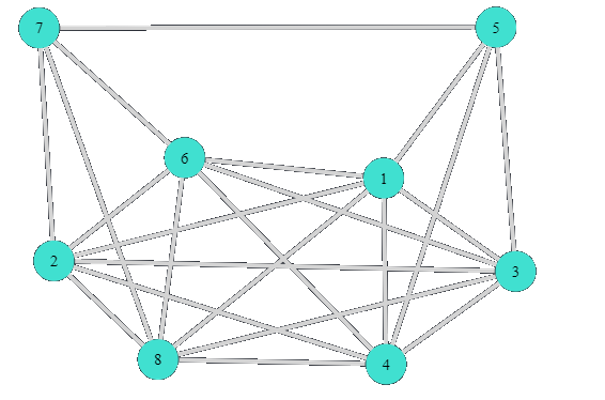
\includegraphics[width=8cm]{Network.png}
%    \caption{Representation of a possible network for eight households}
%    \label{fig:network}
%\end{figure}
\noindent
Note that in this network, not all nodes (which represent households) will be connected to each other, but rather each node will be connected to a selection of different nodes. Based on these connections, households will experience the peer effect. The quantification of the social utility in this setting can be done by using the equation:
\noindent
\begin{equation}
    UT_{soc} = \frac{\#PV}{\#Total}
\end{equation}
Where $\#PV$ is the amount of neighbors a household has that has adopted a PV-battery configuration and $\#Total$ the overall amount of neighbors a certain agent has. The social utility will, therefore, always have a value between 0 and 1. When looking at Figure \ref{fig:network}, the total amount of neighbors can easily be determined by counting the amount of connection that arrive at a certain point. The amount of PV adopters is the central emergent variable in the model and will initially be fuelled by just economic utility, but as adoption increases, so will the social utility and, therefore, the adoption will be fuelled by a mix of economic and social utility.
%\subsubsection{Uncertainty in the ABM}
%Since this model considers investment decisions in DERs, there is going to be a level of uncertainty, since an investment decision will always entail a certain risk. It is, therefore, necessary to introduce some uncertainty in the model. Uncertainty can be incorporated into many aspect of this model:
%\begin{itemize}
%    \item DAM electricity price: By letting the prices vary overtime with some degree %of randomness, uncertainty is introduced into the model.
%    \item Load factor: By letting the load factor fluctuate at random, the production %of the PV becomes uncertain, thereby introducing uncertainty in the model.
%    \item Learning rate technologies: Since the technologies under discussion (PV and %residential batteries) are in a steep growth phase, their prices are still decreasing, but this process still has lots of uncertainty, which could also be used as some form of model uncertainty.
%\end{itemize}
%In this Thesis, the uncertainty in the investment cost is considering the main source of uncertainty. This can be done by considering a set of random projections based on a set of assumptions. Given an average cost decrease ("drift"), there will be a certain random deviation from this path.
\subsubsection{Overall utility}
The overall utility can, finally be computed as:
\begin{equation} \label{totut}
    UT_{tot} = w_{eco}*NUT_{eco} + w_{soc}*UT_{soc}
\end{equation}
With $w_{eco}$ the weighting coefficient for the economic utility and $w_{soc}$ the weighting coefficient for the social utility. Note that these weights are subject to the constraint:
\begin{equation}
    w_{eco} + w_{soc} = 1
\end{equation}
This total utility is to be compared with the adoption threshold of the agent to determine whether the total utility is sufficient to make the household adopt the DERs. These thresholds for different types of households can be found in table \ref{table:threshold}.
\begin{table}[h]
\centering
 \begin{tabular}{||c|c|c||} 
 \hline
 \textbf{Household type} & \textbf{Threshold[-]} & \textbf{Expected payback (years)}\\
 \hline \hline
 Innovators & 0.4 & 16 \\
 Early Adopters &0.5 & 14\\
 Early Majority & 0.6 & 12\\
 Late Majority & 0.7 & 8\\
 Laggards & 0.8 & 6\\
 \hline
 \end{tabular}
 \caption[Overview of the different household thresholds]{Overview of the different household thresholds}
 \label{table:threshold}
\end{table}
\noindent
As mentioned earlier, the utility will mainly consist of economic utility at the beginning of the simulation, when overall adoption is low, but will gradually become a mix of social and economic utility as adoption increases and social utility increases accordingly. It is important to mention that this overall utility is normalised, and will therefore always be between 0 and 1, depending on the weights of the economic and social utility. This is why the thresholds are between 0.4 and 0.8. Note that the values in Table \ref{table:threshold} are estimates since there is no comprehensive literature on the appropriate selection of these values. 
\newline \newline \noindent
Innovators are households that will purchase and install a PV-battery system out of their motivation to adopt new technologies. This motivation will rarely be an economic one, but rather one of social, environmental, cultural or technological standards the household upholds. Their threshold, therefore, is very low, since the innovator does not need any strong economic or social strong incentive to adopt the new technology. Laggards, on the other hand, will not install a new DERs out of any motivation other than a purely utility-based one. Therefore, the overall utility must be high enough to make the laggard adopt the DERs.
\newline 
\newline
\noindent
The question still remains what the distribution is between these different adoption classes. To do so, Rogers' Theory of Innovation Diffusion is used \cite{Rogers}. This theory describes how new technologies or trends get adopted throughout different classes of the population. Note that the terminology used for the different adoption classes (innovators, early adopters, laggards) also comes from this theory. Rogers' research proposes that from a certain population, innovators account for 2.5\% of a population, early adopters for 13.5\%, the early majority 34\%, late majority 34\% and laggards 16\%. %A representation of this distribution for the population in this model can be found in Figure \ref{fig:classes}.
%\begin{figure}[h!]
%    \centering
%    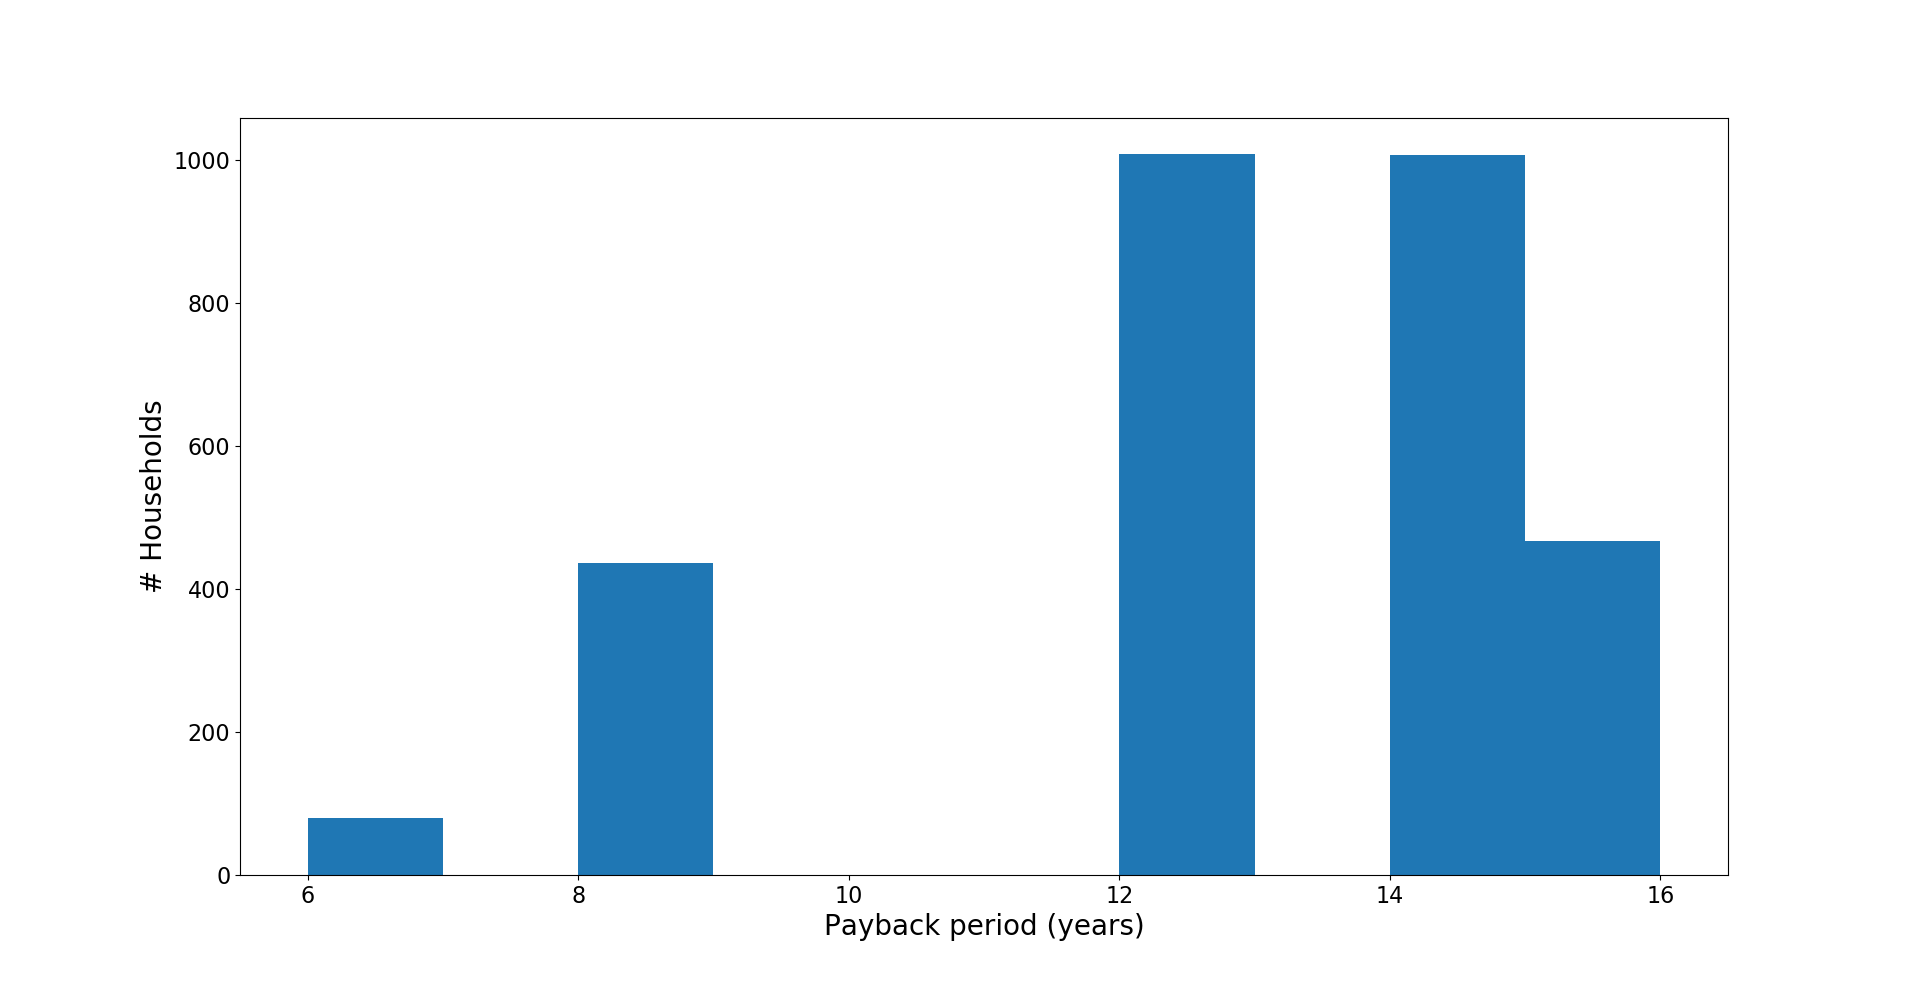
\includegraphics[width=14cm]{Distribution.png}
%    \caption{Distribution of different adoption classes in the model}
%    \label{fig:classes}
%\end{figure}